\chapter{Building Abstractions with Data}

\section{Introduction to Data Abstraction}

\subsection{Example: Arithmetic Operations for Rational Numbers}

\begin{exe}[2.1]
    A possibility for a \vscm{make-rat} handling both positive and negative 
    arguments:
    \scm{ch2/2.01.scm}
\end{exe}

\subsection{Abstraction Barriers}

\begin{exe}[2.2]
    Exemple implementation for the representation of segments in a plane:
    \scm{ch2/2.02.scm}
\end{exe}

\begin{exe}[2.3]
    In the following implementation, a rectangle is represented by its two 
    opposite sides, which must have the same orientation. The code makes use of 
    auxiliary procedures defined below.

    I added selectors to access each of the vertices of the rectangle to be 
    able to print rectangles in a uniform format.
    \scm{ch2/2.03.1.scm}

    The procedures that compute the perimeter and area of a rectangle, and the 
    procedure that prints a rectangle, are defined thus:
    \scm{ch2/2.03.perim-area.scm}

    Another possibility is to represent a rectangle by its four vertices:
    \scm{ch2/2.03.2.scm}

    Yet another possibility is to represent a rectangle by two perpendicular 
    segments with the same origin:
    \scm{ch2/2.03.3.scm}

    The procedures \vscm{perim-rect}, \vscm{area-rect} and \vscm{print-rect} 
    work in all three cases.

    \begin{comp}
        The code above makes use of the following auxiliary procedures to check 
        that the input is correct, compute the length of a segment, and print 
        points inline for use in \vscm{print-rect}:
        \scm{ch2/2.03.aux.scm}
    \end{comp}
\end{exe}

\subsection{What Is Meant by Data?}

\begin{exe}[2.4]
    With the representation of pairs given in the exercise, \vscm{(cons x y)} is 
    a procedure that takes as its argument a procedure \vscm{m} with two 
    arguments and returns the result of the application of \vscm{m} to \vscm{x} 
    and \vscm{y}.

    \vscm{(car z)} applies the procedure \vscm{(cons x y)} to the procedure that 
    returns the first of its arguments, so \vscm{(car (cons x y))} yields 
    \vscm{x}.

    Using the substitution model, the successive steps are:
    \scm{ch2/2.04a.scm}

    The corresponding definition of \vscm{cdr} is:
    \scm{ch2/2.04b.scm}
    The method to prove that \vscm{(cdr (cons x y))} yields \vscm{y} is the same 
    as with \vscm{car}.
\end{exe}

\begin{exe}[2.5]
    If $a$ and $b$ are known, we can compute $2^a 3^b$, and since the 
    decomposition of integers as a product of primes is unique, it’s possible to 
    find $a$ and $b$ from the value of $2^a 3^b$.

    The procedures \vscm{cons}, \vscm{car}, and \vscm{cdr} corresponding to this 
    representation can be defined as:
    \scm{ch2/2.05.scm}
\end{exe}

\begin{exe}[2.6]
    The successive substitution steps to evaluate \vscm{(add-1 zero)} are:
    \scm{ch2/2.06a.scm}

    In other words, \vscm{one} is a procedure that takes a one-argument 
    procedure as its argument and returns it.

    The substitution steps to evaluate \vscm{(add-1 one)} are:
    \scm{ch2/2.06b.scm}

    In other words, \vscm{two} is a procedure that takes a one-argument 
    procedure $f$ as its argument and returns the procedure $f \circ f$ ($f$ 
    applied twice).

    From these observations, and after remarking that \vscm{zero} is a procedure 
    that takes one argument and always returns the identity procedure, we can 
    make the hypothesis that the $n$th Church numeral is a procedure that takes 
    a one-argument procedure $f$ as its argument and returns the $n$th repeated 
    application of $f$ (see exercise~\ref{1.43}). This can be proved by 
    induction.

    \begin{proof}
        We’ve already shown that it’s true for $0$, $1$ and $2$.
        Let’s assume that it’s true for a positive integer $n$.

        From the induction hypothesis, \vscm{(n f)} is the $n$th repeated 
        application of $f$, so it’s obvious that
        \vscm{(lambda (x) (f ((n f) x)))} is the $(n + 1)$th repeatead 
        application of $f$, so the result is true for $n + 1$, hence it’s true 
        for any positive integer $n$.
    \end{proof}

    To apply a function $n + m$ times, we just need to apply it $m$ times, and 
    then $n$ times more, so \vscm{+} can be defined directly as:
    \scm{ch2/2.06c.scm}
\end{exe}

\subsection{Extended Exercise: Interval Arithmetic}

Let’s first define a function that prints intervals:
\scm{ch2/2.07pre2.scm}

\begin{exe}[2.7]
    Since \vscm{make-interval} has been defined as \vscm{cons}, 
    \vscm{upper-bound} and \vscm{lower-bound} can be defined as \vscm{cdr} and 
    \vscm{car} respectively.
    \scm{ch2/2.07.scm}
\end{exe}

\begin{exe}[2.8]
    With the same reasoning as for division, the subtraction of two intervals is 
    the addition of the first with the opposite of the second.
    The subtraction procedure can thus be defined:
    \scm{ch2/2.08.scm}
\end{exe}

\begin{exe}[2.9]
    Let $[a;b]$ and $[c;d]$ be two intervals.

    Their sum is $[a + c; b + d]$. Its width is $\sfrac{(b + d) - (a + c)}{2} 
    = \sfrac{(b - a)}{2} + \sfrac{(d - c)}{2}$, in other words, the sum’s 
    width is the sum of the widths, so it depends only on the widths of the 
    intervals being added.

    The difference can be defined as the sum with the opposite, and taking the 
    opposite doesn’t change the width, so this is also true for differences.

    For multiplication and division, the width of the result also depends on 
    the values of the bounds. For instance, $[1; 2] \times [2; 3] = [2; 6]$, 
    but $[0; 1] \times [2; 3] = [0; 3]$. In both cases, we multiply two 
    intervals of width $\sfrac{1}{2}$, but the former product has a width of 
    $2$ while the latter has a width of $\sfrac{3}{2}$, so the width of the 
    product is not a function of the widths of the intervals being multiplied.

    Since division can be defined as a multiplication, this is also true for 
    division.
\end{exe}

\begin{exe}[2.10]
    The new code of \vscm{div-interval} could be:
    \scm{ch2/2.10.scm}
\end{exe}

\begin{exe}[2.11]
    There are three cases for each interval:
    \begin{itemize}
        \item the lower bound is positive or null;
        \item the upper bound is negative or null;
        \item the lower bound is negative and the upper bound is positive.
    \end{itemize}
    This results in a total of nine cases, and the only case where the smallest 
    and greatest products can’t be deduced from the signs is when both intervals 
    span zero.

    A procedure taking this suggestion into account is:
    \scm{ch2/2.11.scm}
\end{exe}

\begin{exe}[2.12]
    The procedures \vscm{make-center-percent} and \vscm{percent} can be defined 
    as:
    \scm{ch2/2.12.scm}
\end{exe}

\begin{exe}[2.13]
    Let $c_1, c_2, w_1$ and $w_2$ be the centers and widths of two intervals. We 
    assume that all numbers are positive. The lower and upper bounds of the 
    product are
    $(c_1 \pm w_1) \times (c_2 \pm w_2) = c_1 c_2 \pm (c_1 w_2 + c_2 w_1) + w_1 
    w_2$.

    Since the percentages are small, $w_1 w_2$ is negligible, and the product’s 
    width is $w \approx c_1 w_2 + c_2 w_1$.

    Additionally, if we call the percentage tolerances $p_1$ and $p_2$ 
    respectively, we have $w_i = c_i \times \sfrac{p_i}{100}$ for $i = 1, 2$.

    From there, $w \approx c_1 c_2 \times \sfrac{p_1 + p_2}{100}$, and $c_1 c_2$ 
    is the product’s center, so under the given conditions, the approximate 
    percentage tolerance of the product is the sum of the tolerances of the 
    factors.
\end{exe}

\begin{exe}[2.14]
    TODO
\end{exe}

\begin{exe}[2.15]
    TODO
\end{exe}

\begin{exe}[2.16]
    TODO
\end{exe}

\section{Hierarchical Data and the Closure Property}

\subsection{Representing Sequences}

\begin{exe}[2.17]
    The \vscm{last-pair} procedure can be defined as:
    \scm{ch2/2.17.scm}
\end{exe}

\begin{exe}[2.18]
    The \vscm{reverse} procedure can be defined as:
    \scm{ch2/2.18.scm}
\end{exe}

\begin{exe}[2.19]
    The procedures can be defined respectively as \vscm{car}, \vscm{cdr} and 
    \vscm{null?}.
    \scm{ch2/2.19.scm}

    The order of the list \vscm{coin-values} does not affect the answer produced 
    by \vscm{cc}, because \vscm{cc} gives the total number of combinations, and 
    the relation used for the computation does not depend on a particular order.
\end{exe}

\begin{exe}[2.20]
    A possible solution is:
    \scm{ch2/2.20.scm}
\end{exe}

\begin{exe}[2.21]
    The completed procedures are:
    \scm{ch2/2.21.scm}
\end{exe}

\begin{exe}[2.22]
    With the first procedure, the answer list is in reverse order because the 
    elements are added to it starting from the beginning of the initial list, 
    and the first element added to a list is at its end.

    With the second procedure, the result is not a list because \vscm{cons} is 
    called with a list as its first argument and the element to add as its 
    second argument. To add an element to a list, the order of the arguments 
    should be the opposite.
\end{exe}

\begin{exe}[2.23]
    Here is a possible implementation of \vscm{for-each}:
    \scm{ch2/2.23.scm}
\end{exe}

\subsection{Hierarchical Structures}

\begin{exe}[2.24]
    The result given by the interpreter is \vscm{(1 (2 (3 4)))}. To represent 
    the corresponding box-and-pointer structure in terms of pairs, one must use 
    the equality of \vscm{(list 1 (list 2 (list 3 4)))} and
    \vscm{(cons 1 (cons (list 2 (list 3 4)) nil))}, and similar equalities for 
    the two other lists.

    \begin{figure}
        \centering
        \begin{tikzpicture}[box and pointer]
            \matrix[cell matrix] {
            \node[car] (11) {}; & \node[cdr] (12) {}; &[+\boxsize]
            \node[car] (13) {}; & \node[cdr] (14) {}; \\

            \node[box] (1) {1}; &&
            \node[car] (21) {}; & \node[cdr] (22) {}; &[+\boxsize]
            \node[car] (23) {}; & \node[cdr] (24) {}; \\

            &&
            \node[box] (2) {2}; &&
            \node[car] (31) {}; & \node[cdr] (32) {}; &[+\boxsize]
            \node[car] (33) {}; & \node[cdr] (34) {}; \\

            &&&&
            \node[box] (3) {3}; &&[+\boxsize]
            \node[box] (4) {4}; \\
            };

            \link{11}{1}
            \link{12}{13}
            \link{13}{21}
            \link{21}{2}
            \link{22}{23}
            \link{23}{31}
            \link{31}{3}
            \link{32}{33}
            \link{33}{4}
            \nil{14}
            \nil{24}
            \nil{34}
        \end{tikzpicture}
        \caption{Box-and-pointer-structure of \vscm{(1 (2 (3 4)))}.}
    \end{figure}

    \vspace*{1cm}
    \begin{figure}
        \centering
        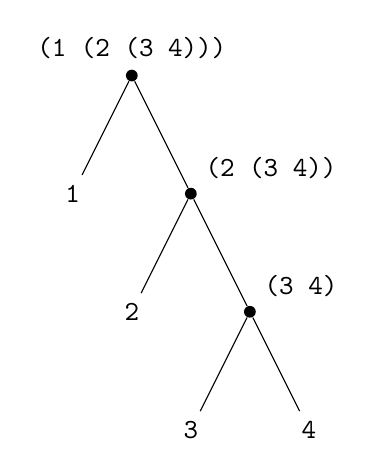
\begin{tikzpicture}[node font=\ttfamily,inner/.style={circle,fill=black, 
        inner sep=1.5pt}]
        \node[inner, label={(1 (2 (3 4)))}] {}
         child { node {1} }
         child { node[inner, label=45:{(2 (3 4))}] {}
             child { node {2} }
             child { node[inner, label=45:{(3 4)}] {}
                child { node {3}}
                child { node {4}}
                }
             };
        \end{tikzpicture}
        \caption{Tree representation of \vscm{(1 (2 (3 4)))}.}
    \end{figure}
\end{exe}

\begin{exe}[2.25]
    If we call the three lists $x$, $y$ and $z$ respectively, the combinations 
    \vscm{(car (cdr (car (cdr (cdr x)))))}, \vscm{(car (car y))} (which can be 
    shortened to \vscm{(caar y)}), and\linebreak
    \vscm{(car (cdr (car (cdr (car (cdr (car (cdr (car (cdr (car (cdr z))))))))))))}
    or, more simply,
    \vscm{(cadr (cadr (cadr (cadr (cadr (cadr z))))))},
    all pick 7 from the lists.
\end{exe}

\begin{exe}[2.26]
    The results printed by the interpreter are \vscm{(1 2 3 4 5 6)} for
    \vscm{(append x y)}, \vscm{((1 2 3) 4 5 6)} for \vscm{(cons x y)} and
    \vscm{((1 2 3) (4 5 6))} for \vscm{(list x y)}.
\end{exe}

\begin{exe}[2.27]
    Here is a possible solution for \vscm{deep-reverse}:
    \scm{ch2/2.27.scm}
\end{exe}

\begin{exe}[2.28]
    A possible solution for \vscm{fringe} is:
    \scm{ch2/2.28.scm}
\end{exe}

\begin{exe}[2.29]
    \ \vspace{-20pt}
    \begin{itemize}
        \item[a.] The selectors can be defined as:
            \scm{ch2/2.29a.scm}
        \item[b.] The total weight can be computed with:
            \scm{ch2/2.29b.scm}
        \item[c.] Since we defined a \vscm{branch-weight} procedure in b., 
            \vscm{balanced?} can be defined simply with:
            \scm{ch2/2.29c.scm}
        \item[d.] To convert to the new representation, the only things that 
            need to be changed are the \vscm{right-branch} and 
            \vscm{branch-structure} selectors:
            \scm{ch2/2.29d.scm}
    \end{itemize}
\end{exe}

\begin{exe}[2.30]
    The two \vscm{square-list} procedures are identical to the \vscm{scale-tree} 
    procedures defined in the text, except that there is only one argument and 
    \vscm{(* tree factor)} is replaced with \vscm{(square tree)}.

    Direct definiton:
    \scm{ch2/2.30a.scm}

    Using \vscm{map} and recursion:
    \scm{ch2/2.30b.scm}
\end{exe}

\begin{exe}[2.31]
    The procedure \vscm{tree-map} can be defined without using \vscm{map}:
    \scm{ch2/2.31a.scm}
    or using it:
    \scm{ch2/2.31b.scm}
\end{exe}

\begin{exe}[2.32]
    The completed procedure is:
    \scm{ch2/2.32.scm}

    The empty set has only one subset: the empty set.

    For a non-empty (finite) set, with elements $\{a_1, …, a_n\}$, the set of 
    subsets is the reunion of the subsets not containing $a_1$ and the subsets 
    containing $a_1$, and the application $S \mapsto S \cup \{a_1\}$ is 
    a bijection between these two sets.
\end{exe}

\subsection{Sequences as Conventional Interfaces}

\subsubsection{Sequence Operations}

\begin{exe}[2.33]
    The operations can be redefined as:
    \scm{ch2/2.33.scm}
\end{exe}

\begin{exe}[2.34]
    A polynomial can be evaluated using Horner’s rule with the procedure:
    \scm{ch2/2.34.scm}
\end{exe}

\begin{exe}[2.35]
    This can be done with or without \vscm{enumate-tree}. Without that function:
    \scm{ch2/2.35.scm}
    The mapped function associates to each subtree its number of leaves: 1 if 
    the subtree has no children, i.e.\ is a leaf, \vscm{(count-leaves subtree)} 
    otherwise.
\end{exe}

\begin{exe}[2.36]
    The procedure \vscm{accumulate-n} can be defined as:
    \scm{ch2/2.36.scm}
\end{exe}

\begin{exe}[2.37]
    The matrix operation can be define as:
    \scm{ch2/2.37.scm}
\end{exe}

\begin{exe}[2.38]
    The value of \vscm{(fold-right / 1 (list 1 2 3))} is $\sfrac{3}{2}$.

    The value of \vscm{(fold-left / 1 (list 1 2 3))} is $\sfrac{1}{6}$.

    The value of \vscm{(fold-right list nil (list 1 2 3))} is the list
    \vscm{(1 (2 (3 nil)))}.

    The value of \vscm{(fold-left list nil (list 1 2 p))} is the list
    \vscm{(((nil 1) 2) 3)}.

    \vscm{fold-right} and \vscm{fold-left} produce the same values for any 
    sequence  if (and only if) \vscm{op} is commutative.

    \begin{proof}
        Suppose \vscm{op} commutative. We’ll show by induction that 
        \vscm{fold-left} and \vscm{fold-right} always produce the same results.

        \vscm{(fold-right op init nil)} and
        \vscm{(fold-left op init nil)} both produce \vscm{init}.

        Let’s assume that \vscm{fold-left} and \vscm{fold-right} produce the 
        same values for any list of length $n \geq 0$. If \vscm{sequence} is 
        a list of length $n + 1$,
        \vscm{(fold-right op init sequence)} equals\linebreak
        \vscm{(op (car sequence) (fold-right op init (cdr sequence)))}, and
        \vscm{(fold-left op init sequence)} equals
        \vscm{(op (fold-left op init (cdr sequence)) (car sequence))}. It 
        follows from the induction hypothesis and the commutativity of \vscm{op} 
        that these two values are equal.

        Hence, by induction, \vscm{fold-left} and \vscm{fold-right} always 
        produce the same results.

        Conversely, if \vscm{op} is not commutative, there exists elements 
        \vscm{a} and \vscm{b} such that \vscm{(op a b)} is different from
        \vscm{(op b a)}, and these expressions are equal respectively to
        \vscm{(fold-left op a (list b))} and to
        \vscm{(fold-right op a (list b))}, so \vscm{fold-left} and 
        \vscm{fold-right} don’t always produce the same values.
    \end{proof}
\end{exe}

\begin{exe}[2.39]
    The procedure \vscm{reverse} can be defined in terms of \vscm{fold-left} and 
    \vscm{fold-right} as:
    \scm{ch2/2.39.scm}
\end{exe}

\subsubsection{Nested Mappings}

\begin{exe}[2.40]
    The procedure \vscm{unique-pairs} and the simplified definition of 
    \vscm{prime-sum-pairs} are:
    \scm{ch2/2.40.scm}
\end{exe}

\begin{exe}[2.41]
    A solution using \vscm{unique-pairs} from the previous exercise:
    \scm{ch2/2.41.scm}
    The triples $(i, j, k)$ are in decreasing order because \vscm{unique-pairs} 
    returns pairs $(j, k)$ with $j > k$.
\end{exe}

\begin{exe}[2.42]
    \label{2.42}
    A possible solution, with a position represented as the list of the numbers 
    of the lines occupied by the queen in each column. The position of the queen 
    in the first column is at the end of the list because the functions are 
    easier to write this way. I removed the \vscm{k} parameter in \vscm{safe?} 
    and \vscm{adjoin-position} because I didn’t need it.
    \scm{ch2/2.42.scm}
\end{exe}

\begin{exe}[2.43]
    In Louis’ program, each call to \vscm{(queen-cols k)} calls 
    \vscm{(queen-cols (- k 1))} 8 times, instead of only one time with the 
    program in exercise \ref{2.42}. Since there are 8 recursion levels, Louis’ 
    program will take about $8^8T$ time to solve the eight-queens puzzle.
\end{exe}

\subsection{Example: A Picture Language}
\label{2.2.4}

\subsubsection{The picture language}

\begin{comp}
    To test the code in this section, it’s necessary to load a module including 
    graphical functions. The solution I chose here is to use DrRacket’s 
    \vscm{graphics.ss} library. It required me to adapt my solution to 
    exercise~\ref{2.46} and to slightly modify the \vscm{segments->painter} to 
    use the given viewport. The code from later exercises is sometimes needed to 
    try out some previous code.

    Code to put at the beginning of the file:
    \scm{ch2/2.44pre2.scm}
\end{comp}

\begin{exe}[2.44]
    The definition of \vscm{up-split} is:
    \scm{ch2/2.44.scm}
\end{exe}

\subsubsection{Higher-order operations}

\begin{exe}[2.45]
    The \vscm{split} procedure can be defined as:
    \scm{ch2/2.45.scm}
\end{exe}

\subsubsection{Frames}

\begin{exe}[2.46]
    \label{2.46}
    A possible solution if we are not using \vscm{graphics.ss}:
    \scm{ch2/2.46a.scm}
    With \vscm{graphics.ss}, we must redefine \vscm{make-vect}, \vscm{xcor-vect} 
    and \vscm{ycor-vect}:
    \scm{ch2/2.46b.scm}
\end{exe}

\begin{exe}[2.47]
    The selectors \vscm{origin-frame} and \vscm{edge1-frame} are the same with 
    both implementations:
    \scm{ch2/2.47a.scm}
    For the first implementation:
    \scm{ch2/2.47b.scm}
    For the second implementation:
    \scm{ch2/2.47c.scm}
\end{exe}

\subsubsection{Painters}

\begin{comp}
    Sligthly modified version of \vscm{segments->painter} for use with 
    \vscm{graphics.ss}:
    \scm{ch2/2.48pre2.scm}
\end{comp}

\begin{exe}[2.48]
    Representation of segments:
    \scm{ch2/2.48.scm}
\end{exe}

\begin{exe}[2.49]
    \ \vspace{-20pt}
    \begin{itemize}
        \item[a.] The painter drawing the outline can be defined as: 
            \scm{ch2/2.49a.scm}
        \item[b.] The painter drawing an “X” can be defined as: 
            \scm{ch2/2.49b.scm}
        \item[c.] The painter drawing a diamond can be defined as: 
            \scm{ch2/2.49c.scm}
        \item[d.] The \vscm{wave} painter can be defined as: \scm{ch2/2.49d.scm}
    \end{itemize}
\end{exe}

\subsubsection{Transforming and combining painters}

\begin{exe}[2.50]
    The given transformations can be defined as:
    \scm{ch2/2.50.scm}
\end{exe}

\begin{exe}[2.51]
    \vscm{below} defined as a procedure analogous to the \vscm{beside} 
    procedure:
    \scm{ch2/2.51a.scm}
    In terms of \vscm{beside} and rotation operations:
    \scm{ch2/2.51b.scm}
\end{exe}

\subsubsection{Levels of language for robust design}

\begin{exe}[2.52]
    \ \vspace{-20pt}
    \begin{itemize}
        \item[a.] Possible modified version of \vscm{wave}:
            \scm{ch2/2.52a.scm}
        \item[b.] Modified \vscm{corner-split}:
            \scm{ch2/2.52b.scm}
        \item[c.] Modified \vscm{square-limit}:
            \scm{ch2/2.52c.scm}
    \end{itemize}
\end{exe}

\section{Symbolic Data}

\subsection{Quotation}

\begin{exe}[2.53]
    Check with an interpreter.
\end{exe}

\begin{exe}[2.54]
    A possible implementation of \vscm{equal?}:
    \scm{ch2/2.54.scm}
\end{exe}

\begin{exe}[2.55]
    The expression \vscm{''abracadabra} is equivalent to
    \vscm{(quote (quote abracadabra))}, which evaluates to
    \vscm{(quote abracadabra)}, an expression whose \vscm{car} is \vscm{quote}.
\end{exe}

\subsection{Example: Symbolic Differentiation}
\label{2.3.2}

\begin{exe}[2.56]
    \label{2.56}
    The modified version of \vscm{deriv} and the procedures 
    \vscm{exponentiation?}, \vscm{base}, \vscm{exponent}, and 
    \vscm{make-exponentiation} can be written as:
    \scm{ch2/2.56.scm}
\end{exe}

\begin{exe}[2.57]
    The \vscm{deriv} procedure always calls \vscm{make-sum} and 
    \vscm{make-product} with only two arguments, so all that’s necessary is to 
    redefine \vscm{augend} and \vscm{multiplicand} as indicated in the text, for 
    instance:
    \scm{ch2/2.57a.scm}

    As a supplement, if we also want to be able to call \vscm{make-sum} and 
    \vscm{make-product} with more than two arguments, we can redefine 
    \vscm{make-sum} and \vscm{make-product} as well:
    \scm{ch2/2.57b.scm}
    These procedures also simplify the result very partially by grouping the 
    numerical arguments together, however expressions such as
    \vscm{(make-sum 'x (make-sum 'y 'x))} or
    \vscm{(make-sum 'x 'y 2 'x)} are not simplified.
\end{exe}

\begin{exe}[2.58]
    \ \vspace{-20pt}
    \begin{itemize}
        \item[a.] It is sufficient to redefine the following procedures:
            \scm{ch2/2.58a.scm}
        \item[b.] The following implementations supports only multiplication and 
            addition and can produce results with unnecessary parentheses.

            It uses several helper procedures:
            \begin{itemize}
                \item \vscm{(elt-or-list elts)} returns the car of elts if elts 
                    is of length 1, and the list elts otherwise.
                \item \vscm{(take-until l elt)} returns a list containing all 
                    the elements of l until the first occurrence of \vscm{elt}, 
                    excluding it. If elt is not contained in the list, the full 
                    list is returned.
                \item \vscm{(intersperse l sep)} returns a list containing all 
                    the elements of l, with sep inserted between each pair of 
                    elements.
            \end{itemize}
            \scm{ch2/2.58b.scm}
    \end{itemize}
\end{exe}

\subsection{Example: Representing sets}
\label{2.3.3}

\subsubsection{Sets as unordered lists}

\begin{exe}[2.59]
    The \vscm{union-set} operation can be defined as:
    \scm{ch2/2.59.scm}
\end{exe}

\begin{exe}[2.60]
    If duplicate elements are allowed, we can redefine \vscm{adjoin-set} and 
    \vscm{union-set} in a more efficient way:
    \scm{ch2/2.60.scm}
    The operation \vscm{adjoin-set} now has $\Theta(1)$ complexity, while 
    \vscm{union-set} has $\Theta(n)$ complexity. It’s not possible to improve 
    the performance of \vscm{element-of-set?} and \vscm{intersection-set}.

    This representation would be preferable to the non-duplicate one when there 
    is no need to worry about the size taken by the sets in memory, and when the 
    operations \vscm{adjoin-set} and \vscm{union-set} are used a lot more than 
    \vscm{element-of-set?} and \vscm{intersection-set}.
\end{exe}

\subsubsection{Sets as ordered lists}

\begin{exe}[2.61]
    A possible implementation of \vscm{adjoin-set} requiring on average half as 
    many steps as with the unordered representation is:
    \scm{ch2/2.61.scm}
\end{exe}

\begin{exe}[2.62]
    By using the same method as for \vscm{intersection-set}, we get 
    a $\Theta(n)$ \vscm{union-set} implementation:
    \scm{ch2/2.62.scm}
\end{exe}

\subsubsection{Sets as binary trees}

\begin{exe}[2.63]
    \ \vspace{-20pt}
    \begin{itemize}
        \item[a.] Both procedures produce the same result for every tree. They 
            produce the ordered list representation of the set represented by 
            the tree. For the trees in figure 2.16, they produce the list 
            \vscm{(1 3 5 7 9 11)}.
        \item[b.] If $T(n)$ is the number of steps required to convert 
            a balanced tree to a list, with the first procedure we have: $T(n) 
            \approx 2T\left(\sfrac{n}{2}\right) + \sfrac{n}{2}$ since 
            \vscm{append} has linear complexity. By applying this formula 
            recursively, we can see that $T(n) \approx n +  \sfrac{n \log 
            n}{2}$, so that \vscm{tree->list-1} grows as $\Theta(n \log{n})$.

            With the second procedure, we have $T(n) = 2T(\sfrac{n}{2}) + 1$, so 
            \vscm{tree->list-2} grows as $\Theta(n)$.
    \end{itemize}
\end{exe}

\begin{exe}[2.64]
    \ \vspace{-20pt}
    \begin{itemize}
        \item[a.] If $n = 0$, the constructed tree is empty.

            Otherwise, one element will be the tree’s entry, so $n - 1$ elements 
            will be in the subtrees.
            $l = \lfloor \sfrac{n - 1}{2}\rfloor$ elements are put in the left 
            tree, and the remaining $r = n - 1 - l$ are put in the right tree.

            Since the list is ordered and the elements in the left tree must be 
            smaller than the entry, the first elements of the list are used to 
            build the left tree. The first remaining element is the entry, and 
            the $r$ following remaining elements are used to build the right 
            tree. The remaining elements of this last operation are also the 
            remaining elements for the current call to \vscm{partial-tree}, so 
            all that remains to be done is to put all the results together.

        \item[b.] For \vscm{partial-tree}, the number of steps $T(n)$ as 
            a function of the size of the tree to build $n$ verifies
            $T(n) \approx 2 T\left(\sfrac{n}{2}\right)$, so its growth is in 
            $\Theta(n)$, so \vscm{list->tree} has linear growth.
    \end{itemize}
\end{exe}

\begin{exe}[2.65]
    If we call \vscm{union-set-ordered-list} and 
    \vscm{intersection-set-ordered-list} the linear union and intersection 
    procedures defined for ordered lists, we can define linear procedures 
    \vscm{union-set} and \vscm{intersection-set} for binary trees as:
    \scm{ch2/2.65.scm}
\end{exe}

\subsubsection{Sets and information retrieval}

\begin{exe}[2.66]
    The procedure is almost the same as \vscm{element-of-set?} for sets 
    represented as binary trees:
    \scm{ch2/2.66.scm}
\end{exe}

\subsection{Example: Huffman Encoding Trees}

\begin{exe}[2.67]
    The encoded string is ADABBCA.
\end{exe}

\begin{exe}[2.68]
    \label{2.68}
    A possible implementation of \vscm{encode-symbol} is:
    \scm{ch2/2.68.scm}
\end{exe}

\begin{exe}[2.69]
    A possible implementation for \vscm{successive-merge} is:
    \scm{ch2/2.69.scm}
\end{exe}

\begin{exe}[2.70]
    With a Huffman encoding tree, 84 bits are required for encoding.
    With a fixed-length code, at least 3 bits per symbol are required for an 
    alphabet of 8 symbols, and the message contains 36 symbols, so at least 108 
    bits would have been needed.
\end{exe}

\begin{exe}[2.71]
    \label{2.71}
    Since $\sum_{i = 0}^{k} 2^i = 2^{k + 1} - 1$, every right (or every left) 
    branch of the tree is a leaf, and the tree has a depth of $n - 1$. So the 
    most frequent symbol is encoded with 1 bit, while the least frequent symbol 
    is encoded with $n - 1$ bits.
\end{exe}

\begin{exe}[2.72]
    In the \vscm{encode-symbol} procedure given in exercise \ref{2.68}, only the 
    symbol list of the left subtree is searched at each node encountered, so we 
    can distinguish two cases for the distribution given in exercise \ref{2.71}:

    \paragraph*{The left subtree of each node corresponds to the most frequent 
    symbol.}
    Encoding the most frequent symbol takes $\Theta(1)$ steps since only 
    one search in a list of size one is necessary before a leaf is reached.

    Encoding the least frequent symbol takes $\Theta(n)$ steps, since 
    all the levels of the tree are traversed, and at each level a search in 
    a list of one element is performed.

    \paragraph*{The right subtree of each node corresponds to the most frequent 
    symbol.}
    Encoding the most frequent symbol takes $\Theta(n)$ steps, for the search in 
    the symbol list.

    For the least frequent symbol, at each of the $n - 1$ tree levels the left 
    subtree’s symbol list is searched, which takes $n - 1 - i$ steps, where $i$ 
    is the level number, with $0$ designing the tree root. The number of steps 
    required grows as $\sum_{k = 1}^{n - 1} k = \sfrac{n (n - 1)}{2}$, so the 
    number of steps required to encode the least frequent symbol is in 
    $\Theta(n^2)$.
\end{exe}

\section{Multiple Representations for Abstract Data}

\subsection{Representations for Complex Numbers}

This subsection contains no exercises.

\subsection{Tagged data}

This subsection contains no exercises.

\subsection{Data-Directed Programming and Additivity}

\begin{exe}[2.73]
    \label{2.73}
    \ \vspace{-20pt}
    \begin{itemize}
        \item[a.] \vscm{same-variable?} and \vscm{number?} can’t be integrated 
            to the main dispatch because when they are true, \vscm{exp} has no 
            operator or operands.

        \item[b.] The procedures for derivation can be written in the following 
            way, using \vscm{make-sum} and \vscm{make-product} from section 
            \ref{2.3.2}.
            \scm{ch2/2.73b.scm}

        \item[c.] To allow differentiation of exponents, it’s enough to call the 
            following procedure, using \vscm{make-exporentiation} from exercise 
            \ref{2.56}.

        \item[d.] The only change required is to exchange the arguments when 
            calling \vscm{put}, using e.g. \vscm{(put '+ 'deriv deriv-sum)} 
            instead of \vscm{(put 'deriv '+ deriv-sum)}.
    \end{itemize}
\end{exe}

\begin{exe}[2.74]
    \ \vspace{-20pt}
    \begin{itemize}
        \item[a.] The \vscm{get-record} procedure can be written using 
            \vscm{apply-generic}, provided each division file is tagged with 
            a division-specific tag, and each division has recorded a procedure 
            get-record that takes a file’s contents and returns a procedure 
            returning a given employee’s record.
            \scm{ch2/2.74a.scm}
        \item[b.] \vscm{get-salary} can also be implemented with 
            \vscm{apply-generic}, if each record is tagged with the 
            division-specific tag, and each division records a procedure for the 
            \vscm{get-salary} operation.
            \scm{ch2/2.74b.scm}
        \item[c.] The \vscm{find-employee-record} procedure can be written as:
            \scm{ch2/2.74c.scm}
        \item[d.] When Insatiable takes over a new company, the new company must 
            tag its record file and each of its employee’s record with 
            a specific tag. It must install specific procedures for 
            \vscm{get-record}, \vscm{get-salary}, etc. into the 
            operation-and-type table.
    \end{itemize}
\end{exe}

\subsubsection{Message passing}

\begin{exe}[2.75]
    The constructor \vscm{make-from-mag-ang} can be defined as follows:
    \scm{ch2/2.75.scm}
\end{exe}

\begin{exe}[2.76]
    With generic operations with explicit dispatch, when a new type is added, 
    all existing operations must be updated. When a new operation is added, no 
    change to existing code is required.

    With data-directed style, when a new type is added, all the operations for 
    this type must be added to the table. When a new operation is added, it must be 
    defined and inserted into the table for each type.

    With message-passing, when a new type is added, no change is required to 
    existing code. When a new operation is added, it must be added to all the 
    existing types.

    \medskip

    For a system in which new types must often be added, message-passing is most 
    appropriate. If new operations must often be added, explicit dispatch is 
    most appropriate.
\end{exe}

\section{Systems with Generic Operations}

\subsection{Generic Arithmetic Operations}

\begin{exe}[2.77]
    When one of the generic operations is called on a \vscm{complex} number, 
    \vscm{apply-generic} is called and dispatches the call to the same generic 
    operation on the \vscm{polar} or \vscm{rectangular} number contained in the 
    \vscm{complex}.

    For the object \vscm{z} given in figure 2.24, the procedures called are:
    \begin{cscm}
        (magnitude z)
        (apply-generic 'magnitude z)
        (magnitude (contents z))
        (apply-generic 'magnitude (contents z))
        (magnitude-rectangular (3 . 4))
    \end{cscm}
    So \vscm{apply-generic} is called twice, it dispatches first to the same 
    generic operation \vscm{magnitude}, then to the specific operation for 
    rectangular numbers.
\end{exe}

\begin{exe}[2.78]
    The definitions of \vscm{type-tag}, \vscm{contents} and \vscm{attach-tag} 
    can be modified in the following way to represent ordinary numbers simply as 
    Scheme numbers.
    \scm{ch2/2.78.scm}
\end{exe}

\begin{exe}[2.79]
    To define the \vscm{equ?} procedure, we first define it as a generic 
    operation:
    \scm{ch2/2.79a.scm}
    Then we add the following respectively to the Scheme number, rational and 
    complex packages:
    \scm{ch2/2.79b.scm}
\end{exe}

\begin{exe}[2.80]
    The definition of \vscm{=zero?} is very similar to that of \vscm{equ?}, 
    first define it as a generic operation, then add the necessary code to the 
    Scheme number, rational and complex packages.
    \scm{ch2/2.80.scm}
\end{exe}

\subsection{Combining Data of Different Types}

\begin{exe}[2.81]
    \ \vspace{-20pt}
    \begin{itemize}
        \item[a.] With Louis’s coercion procedures installed, if 
            \vscm{apply-generic} is called with two arguments of type 
            \vscm{complex} for an operation that is not found in the table for 
            those types, as in the example given for \vscm{exp}, 
            \vscm{apply-generic} is called recursively with the same arguments, 
            so there is an infinite loop.
        \item[b.]The  \vscm{apply-coercion} procedure works correctly, however, 
            it’s unnecessary to attempt coercion to the same type so it should 
            not be attempted.
        \item[c.] The new version of \vscm{apply-generic} could be:
            \scm{ch2/2.81.scm}
    \end{itemize}
\end{exe}

\begin{exe}[2.82]
    A version of \vscm{apply-generic} that handles coercion in the case of 
    multiple arguments can look like:
    \scm{ch2/2.82.scm}

    The strategy proposed is not sufficiently general: let’s assume we define 
    a procedure \vscm{exp} for arguments of type \vscm{complex} and 
    \vscm{scheme-number}. If we call it with a rational and a Scheme number, the 
    procedure above will try to coerce both arguments to rationals, and then to 
    Scheme numbers, and will not find a suitable procedure in either case. 
    However, it would have been enough to coerce the first argument to a complex 
    to be able to apply the registered procedure.
\end{exe}

\begin{exe}[2.83]
    \label{2.83}
    The \vscm{raise} operation can be installed with:
    \scm{ch2/2.83.scm}

    \begin{comp}
        So far, we have only used the types \vscm{scheme-number}, 
        \vscm{rational} and \vscm{complex}. Since a lot of Scheme 
        implementations --- including Gambit --- provide the full numeric tower, 
        including predicates \vscm{integer?} and \vscm{real?}, we can implement 
        the full tower by loading the following code:
        \scm{ch2/2.83pre.scm}
    \end{comp}
\end{exe}

\begin{exe}[2.84]
    The \vscm{apply-generic} procedure can be modified as shown below. To add 
    a new level to the tower, in addition to defining the procedures for the new 
    type, the only necessary change is to add the new level to the tower.
    \scm{ch2/2.84.scm}
\end{exe}

\begin{exe}[2.85]
    Let’s first define the \vscm{project} and \vscm{drop} procedures:
    \scm{ch2/2.85a.scm}
    Since \vscm{raise} is defined with \vscm{apply-generic}, simply calling 
    \vscm{drop} after applying the procedure found causes an infinite loop. It’s 
    also unnecessary to call it after \vscm{project}, and it can be called only 
    on results representing numbers. So we add entries in the table to indicate 
    that \vscm{drop} should not be called if the operation applied is 
    \vscm{raise}, \vscm{project}, \vscm{equ?} or \vscm{=zero?}. It is called by 
    default.
    \scm{ch2/2.85b.scm}
\end{exe}

\begin{exe}[2.86]
    The only change required is to use generic operations for all operations on 
    numbers used in the complex, rectangular and polar packages. The generic 
    operations \vscm{add}, \vscm{sub}, \vscm{mul} and \vscm{div} have already 
    been defined, and it’s necessary to define generic operations for 
    \vscm{cos}, \vscm{sin}, \vscm{atan}, \vscm{sqrt} and \vscm{square}.
    \scm{ch2/2.86.scm}
\end{exe}

\subsection{Example: Symbolic Algebra}

\subsubsection{Arithmetic on polynomials}

\begin{comp}
    I decided to add the polynomial type to the tower of types used since 
    exercise \ref{2.83}. For this to work, I had to redefine the tower of types:
    \begin{cscm}
        (define tower '(integer rational real complex polynomial))
    \end{cscm}
    and to define the procedures \vscm{project} and \vscm{equ?} for polynomials, 
    as well as a \vscm{raise} procedure that transforms a complex number into 
    a polynomial of degree 0. So I added the following code to the polynomial 
    package given in the book. This still needs the \vscm{=zero?} procedure 
    defined in the following exercise for \vscm{=equ?} to work on polynomials 
    with polynomial coefficients.
    \scm{ch2/poly-sup.scm}
\end{comp}

\begin{exe}[2.87]
    The \vscm{=zero?} procedure can be defined by adding the following code to 
    the polynomial package:
    \scm{ch2/2.87a.scm}
    \scm{ch2/2.87b.scm}
\end{exe}

\begin{exe}[2.88]
    We can define a generic negation operation \vscm{neg} for types other than 
    polynomial with the following code:
    \scm{ch2/2.88a.scm}
    Then, the \vscm{neg} and \vscm{sub} operations can be implemented for 
    polynomials by adding the following to the polynomial package:
    \scm{ch2/2.88b.scm}
    \scm{ch2/2.88c.scm}
\end{exe}

\begin{exe}[2.89]
    The only procedures that need to be redefined to implement the term-list 
    representation appropriate for dense polynomials are \vscm{adjoin-term} and 
    \vscm{first-term}:
    \scm{ch2/2.89.scm}
\end{exe}

\begin{exe}[2.90]
    I defined two packages to install the representions for the two kinds of 
    term lists. Each package defines \vscm{adjoin-term}, \vscm{first-term}, 
    \vscm{rest-terms}, \vscm{empty-termlist?}, as well as a constructor for the 
    empty term list.

    For the \vscm{adjoin-term} procedure, a generic procedure on the kind of 
    term-list returns a lambda that takes a term as an argument. This avoids 
    having to tag the term as well.

    The procedures \vscm{coeff}, \vscm{order} and \vscm{make-term} have been put 
    out of the polynomial package because they are needed in all three packages.

    The only adaptation needed for the other procedures of the polynomial 
    package is to replace calls to \vscm{(the-empty-termlist)} with calls to 
    \vscm{make-empty-termlist} with the correct type. For simplicity, I used the 
    type of the arguments rather than looking at the number of non-zero 
    coefficients of the result to pick the best representation.
    \scm{ch2/2.90.scm}
\end{exe}

\begin{exe}[2.91]
    The \vscm{div-poly} and \vscm{div-terms} procedures can be defined in the 
    following way. I used the polynomial package with two term-list 
    representations from the previous exercise. For testing, I added
    \vscm{(put 'no-drop? 'div true)} to prevent \vscm{apply-generic} from 
    attempting to simplify the list of two polynomials returned by the division, 
    but it would be better to modify the way \vscm{apply-generic} decides 
    whether to simplify its results to avoid disabling simplification entirely.
    \scm{ch2/2.91a.scm}
    \scm{ch2/2.91b.scm}
\end{exe}

\subsubsection{Hierarchies of types in symbolic algebra}

\begin{exe}[2.92]
    I tried to find a solution that was as general as possible: works for an 
    arbitrary number of variables used in the polynomials, in any order. The 
    variables are ordered alphabetically.

    The \vscm{poly->monoms} procedure transforms a polynomial into an ordered 
    list of monoms. A monom consists of a list of variable-power lists and 
    a non-zero coefficient.
    The order on the variable-power lists is defined by:
    \vscm{(< (var1 n1) (var2 n2))} iff
    \begin{cscm}
    (or (string<? var1 var2)
        (and (string=? var1 var2) (> n1 n2)))
    \end{cscm}
    (where we omitted the calls to \vscm{symbol->string} for simplicity.
    The monoms are ordered lexicographically on their lists of variables, with 
    the empty list appearing last.

    The \vscm{monoms->poly} procedure transforms the list of monoms built by 
    \vscm{poly->monoms} back into a polynomial where each variable appears only 
    at one level, and the variables appear in alphabetical order. Note that 
    \vscm{monoms->poly} can actually return types other than polynomial, if the 
    original polynomial was of degree 0.

    The \vscm{make-same-var} procedure takes two polynomials and returns a pair 
    of two polynomials in the same main variable. This is useful if the 
    variables appearing in the two polynomials are different. If the same 
    variables appear, but ordered differently, \vscm{monoms->poly} is enough.

    Since \vscm{monoms->poly} can return types other than polynomial, it must 
    return tagged data, and \vscm{add-poly}, \vscm{mul-poly}, \vscm{neg-poly} 
    and \vscm{div-poly} have been transformed to return tagged data as well.

    \begin{comp}
        I kept the original code in the case when the two polynomials are in the 
        same variable, but in the case that, say, p1 is a polynomial in $x$ with 
        coefficients in $y$, some of them having coefficients in $x$ as well, this 
        won’t work and the transformation to a canonical form should be used. We’ll 
        assume that this doesn’t happen to avoid going through the transformation 
        when it’s not necessary.

        It would also have been possible to rewrite \vscm{add-poly} and 
        \vscm{mul-poly} so that the operations are made on the monoms rather than 
        the terms, e.g. two polynomials can be added with:
        \begin{cscm}
            (monoms->poly (merge-monoms (poly->monoms p1)
            (poly->monoms p2)))
        \end{cscm}
    \end{comp}

    Additions to the polynomial package:
    \scm{ch2/2.92.scm}
    Changes to existing code:
    \scm{ch2/2.92changes.scm}
\end{exe}

\subsubsection{Extended exercise: Rational functions}

\begin{exe}[2.93]
    The changes to the rational packages are straightforward.
    \scm{ch2/2.93.scm}

    \begin{comp}
        In order to continue to use all the fonctionalities defined in the 
        exercises in the chapter, I had to modify the procedures defining 
        \vscm{project} and \vscm{equ?} for rationals.
        \scm{ch2/2.93sup.scm}
    \end{comp}
\end{exe}

\begin{exe}[2.94]
    The procedures \vscm{remainder-terms} and \vscm{gcd-poly} can be implemented 
    in the following way:
    \scm{ch2/2.94.scm}
\end{exe}

\begin{exe}[2.95]
    \label{2.95}
    Dividing by hand, the remainder found after the first division is
    $\sfrac{1458}{169} x^2 - \sfrac{2916}{169} x + \sfrac{1458}{169}$, which 
    divides $Q_2$.

    With Gambit scheme, the first remainder is a polynomial with 
    limited-precision decimal numbers as coefficients, and the second call does not 
    return.
\end{exe}

\begin{exe}[2.96]
    \ \vspace{-20pt}
    \begin{itemize}
        \item[a.] The procedure \vscm{pseudoremainder-terms} can be defined as:
            \scm{ch2/2.96a1.scm}
            and the new version of \vscm{gcd-terms} is:
            \scm{ch2/2.96a2.scm}
            On the example in exercise \ref{2.95}, 
            \vscm{greatest-common-divisor} now produces the polynomial $1458 x^2 
            - 2916 x + 1458$.
        \item[b.] The procedure can be rewritten in the following way to divide 
            the coefficients of the answer by their greatest common divisor.
            \scm{ch2/2.96b.scm}
    \end{itemize}
\end{exe}

\begin{exe}[2.97]
    \ \vspace{-20pt}
    \begin{itemize}
        \item[a.] The \vscm{reduce-terms} and \vscm{reduce-poly} procedures can 
            be defined as:
            \scm{ch2/2.97a.scm}
        \item[b.] The only change needed besides adding the necessary entries to 
            the associative table is to redefine \vscm{make-rat} as:
            \scm{ch2/2.97b.scm}
            The result returned by \vscm{(add rf1 rf2)} corresponds to
            $\frac{-x^3 - 2x^2 - 3x - 1}{-x^4 - x^3 + x + 1}$, which is 
            correctly reduced to lowest terms, though multiplying both the 
            numerator and the denominator by $-1$ would seem more natural.
    \end{itemize}
\end{exe}
